%%%%%%%%%%%%%%%%%%%%%%%%%%%%%%%%%%%%%%%%%%%%%%%%%%%%%%%%%%%%%%%%%%%%%%%%%%%%%%%%
%2345678901234567890123456789012345678901234567890123456789012345678901234567890
%        1         2         3         4         5         6         7         8
% THESIS CHAPTER

\chapter{Evaluation benchmark}
\label{chap:benchmark}
\ifpdf
    \graphicspath{{Algorithms/Figures/PNG/}{EvaluationTask/Figures/PDF/}{Algorithms/Figures/}}
\else
    \graphicspath{{Algorithms/Figures/EPS/}{EvaluationTask/Figures/}}
\fi


% short summary of the chapter

The benchmark implementing the algorithm was targeted for solely personal use,
therefore the majority of its functionality is not easily accessible through a
form of a user interface. The output that most functions generate is verbose and
is intended to assist with the analysis of the inner workings of an algorithm.
Overall it is recommended the benchmark to be used as a software library, rather
than a standalone tool.

Following on the design of the evaluation task any usage of the benchmark
requires a MongoDB instance to store audio features and act as a song
database on figure \ref{fig:bencharch}. A Docker Compose recipe is available in
the \textit{misc/docker} directory of the project GitLab repository for quick
spawning a MongoDB container.

\section{Implementation details} 
\label{sec:implementation}

As mentioned before the whole benchmark is implemented in Python 3.7. To perform
audio feature extraction from a song the benchmark utilises Librosa, a library
for  audio and music processing \cite{librosa}. Librosa offers various functions
to extract all required audio features using different Fourier transforms, as
well as the ability to separate a song into beat frames. The software was also
written by the authors of the cross-correlation rejector \cite{ellis2008cross},
and its beat tracker implementation is the core of beat tracking for the timbre
rejector implementation \cite{tralie2015cover}. Because of that Librosa was
the preferred choice for audio analysis library over other options \cite{aubio}
\cite{pyAudioAnalysis}.

Connections between the benchmark and the database are accommodated
through the official MongoDB Python package called \textit{PyMongo}
\cite{pymongo}. The audio feature extraction functionality in the benchmark
could potentially serve as a middleware between Librosa and PyMongo in future
MIR-related projects.

Other general matrix operations are achieved using \textit{NumPy}, a popular
scientific computation Python package \cite{numpy}.

The benchmark is mainly targeted to be run on sets of query songs, rather than
individual songs. Each algorithm implementation however has a
\textit{run\_on\_test\_set} and \textit{run\_on\_query\_song} functions, which
initiate an algorithm runs on a set of query songs or an individual query track.

\section{Algorithm implementations in the benchmark} 
\label{sec:algostructure}
This section offers documentation on the exact parameters used during each
algorithm implementation. It complements all information from chapter
\ref{chap:algorithms}. 
\subsection{Weak rejectors}
\label{subsec:weakrejectorimplementation}
Tempo, loudness and duration weak rejectors have been produced by the benchmark.
Each rejector is in the form of a classifier model, with an implementation for
ExtraTrees classification provided by the \textit{scikit-learn} Python library
\cite{scikit-learn}. The trained models are stored into the database, so that
they can be reused to produce classifications during an algorithm execution. The
maximum depth for each tree in the model is set to 20. Due to memory concerns
the classifier is trained using batches of data rather than on the full training
set at the same time. A tree is added for each training phase using a batch of
data. For batches of approximately 42,000 pairs the overall number of trees in
the trained model is 1819. The low maximum depth of a tree combined with the
number of trees helps reduce model overfitting \cite{osmalsky2016enhancing}.

The ROC scores returned by the trained models used in the results generation are
$0.5$ for the duration and tempo classifiers and $0.53$ for the loudness
classifier.

\subsection{Cross-correlation rejector}
\label{subsec:ccsimplementation}

Chroma features for the cross-correlation rejector are extracted using STFT with
a window size of 2048 samples and a hop length of 512 samples. The extraction of
the beat frames of a song is done using an initial tempo estimate of 240 beats
per minute (bpm), a value mentioned in the original algorithm implementation.
The cross-correlation of two chromagrams is performed on row pairings using the
NumPy \textit{correlate} function. The resulting cross-correlation matrix is
normalised by the size of the smaller chromagram so that the maximum possible
peak value is 1.

\subsection{Quantisation rejector}
\label{subsec:quantisationimplementation}

The process of extracting chroma vectors in the quantisation rejector is
completely identical to the cross-correlation rejector implementation. The
trained K-means model forms 200 cluster centers and uses \textit{k-means++}
(initial random selection of first cluster center with every following center
selected using a weighted probability based on distance to all previously chosen
centers) as an initialisation model. The K-Means clustering implementation was
provided by scikit-learn. The training phase involved approximately 42,000
chroma vectors extracted from the train sets of the datasets. The finalised
model is again stored into the database for persistence.

The achieved inertia of the best performing K-means model was 5633.

\subsection{Timbre rejector}
\label{subsec:timbreimplementation}

The extraction of MFCCs for the timbre rejector was achieved through the
\textit{mfcc} function provided by Librosa, which inherently uses a discrete
cosine transform (DCT), a Fourier-related transform similar to DFT. The window
size of the transform is dependent on the tempo of a song and is determined by
the function $\frac{60}{tempo} * sr$, where $sr$ is the sample rate of the song.

The beat tracking takes 3 initial guesses for tempo (60, 100, 180) and 3
dimensions (100 $\times$ 100, 200 $\times$ 200, 300 $\times$ 300) are examined
for size of the self-similarity matrix for each track. This leads to the
construction of 9 self-similarity matrices (SSMs) for each database or query song.

An implementation of the Smith-Waterman algorithm provided by the creator of the
algorithm is directly used to generate similarity scores.

The current version of the timbre rejector runs considerably slower compared to
the other audio similarity algorithms. While a run of the rest of the algorithms
usually takes a relatively short time (up to 30 minutes per dataset) the
timbre-based algorithm takes a variable time between 2 and 6 hours to return a
result for a single query song of the dataset. A potential reason for the long
run time could be the high computational costs associated with handling 9 SSM
representations for a single database song. Each SSM represented as a NumPy
matrix takes a lot of storage space - the total size of the SSMs for all
database songs for the \textit{covers80} dataset takes almost 90 GB in MongoDB.
Retrieving such a significant amount of data from the database for every query
song, combined with the construction of a cross-similarity matrix for each SSM
results in a very slow task. Even utilising lazy loading, a pre-processing step
required due to all SSM results from the database being too big to fit in
memory, does not result in any noticeable improvement of the time for execution.


% Make sure to mention and make a discussion on why the timbre rejector runs slow

\subsection{Rank aggregation rejector}
\label{subsec:rankaggrimplementation}
The rank aggregation rejector takes advantage of the \textit{min, max, median}
and \textit{mean} functions in NumPy to determine an aggregated rank from an
array of ranks.

\subsection{Fingerprint rejector}
\label{subsec:fingerprintimplmentation}

As per algorithm specification, the constant Q transform (CQT) applied on query
segments and database songs uses a window size of 512 samples, a range of 120
frequency channels and a minimum frequency of 130.81 Hz (equivalent to the C3
note). The conversion of the resulting spectrogram to a binary image is
performed using a adaptive thresholding implementation provided by the
\text{scikit-image}, a Python image processing library. The neighbourhood sizes
considered are 15 and 35. Hamming similarity is calculated using the
\textit{hamming} function from \textit{SciPy}, another scientific calculation
package. 

\section{Benchmark result format} 
\label{sec:resformat}

The result of an algorithm run on a query song is stored as an entry in a
MongoDB collection. Apart from the actual similarity scores each entry also
includes metadata allowing for easy understanding of the results:

\begin{figure}[H]
   \centering 
   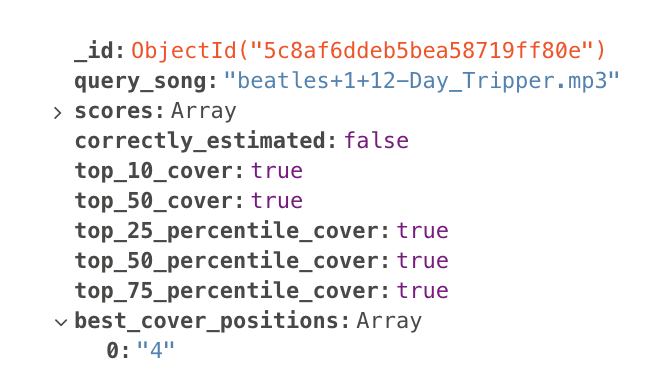
\includegraphics[width=0.5\textwidth]{Benchmark/overallresult.png}
   \captionof{figure}[Example of an algorithm result in database]{An example of an algorithm result for a single query song. The representation accommodates for a quick retrieval of the \textit{Top-K} and \textit{Text-P} evaluation metrics}
   \label{fig:overallresult}
\end{figure}

The verbose similarity scores are available in the \textit{scores} array:

\begin{figure}[H]
    \centering
    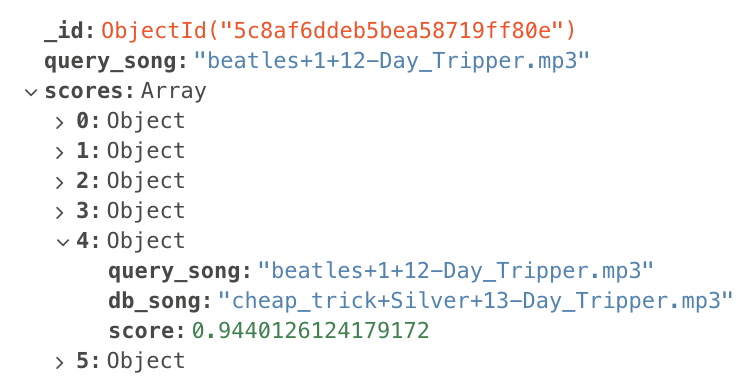
\includegraphics[width=0.5\textwidth]{Benchmark/scoresresult.png}
    \captionof{figure}[Example of verbose similarity score in database]{Verbose scores stored in the database}
    \label{fig:scoresresult}
\end{figure}

The benchmark supports exporting the evaluation metrics defined in chapter
\ref{chap:task} as CSV files.